% !TEX root = ./../../_Thesis.tex

% chapter's came and label
\chapter{Related Work}
\label{chap:RelatedWork}

Vision simulation has been addressed in different ways over the years. Since 
%1981, when 
the first synthetic image with depth of field computed by \citet{Potmesil1981}, there has been a significant number of computer graphics techniques addressing the rendering of realistic effects. More recently, the possibility of estimating and compensating for refractive errors has attracted the attention of several researchers, mainly addressing the formulation of interactive, portable, and inexpensive solutions. The following subsections describe the main techniques for simulating, estimating, and correcting visual aberrations.

% Visual Simulation Section
% !TEX root = ./../../_Thesis.tex

% section's Name and Label
\section{Visual Simulation}
\label{sec:VisualSimulation}

%Lorem ipsum dolor sit amet, consectetur adipiscing elit.

	% Optical Simulation Techniques Section
	% !TEX root = ./../../_Thesis.tex

% section's Name and Label
\subsection{Optical Simulation Techniques}
\label{subsec:OpticalSimulationTechniques}

\citet{Barsky2004} proposed a method for generating synthetic images incorporating the optical characteristics of an individual. Specifically, his method simulates the perception of an individual based on data acquired using a Shack-Hartmann wavefront aberrometer. Figure \ref{fig:barsky_algorithm} shows a rendered image using his technique, along with an overview of the algorithm. Note that once the wavefront data is captured, it is sampled to calculate an {\it Object Space PSF} (OSPSF) and used to blur the input synthetic scene at different depths.

\begin{figure}[h]

	\centering
	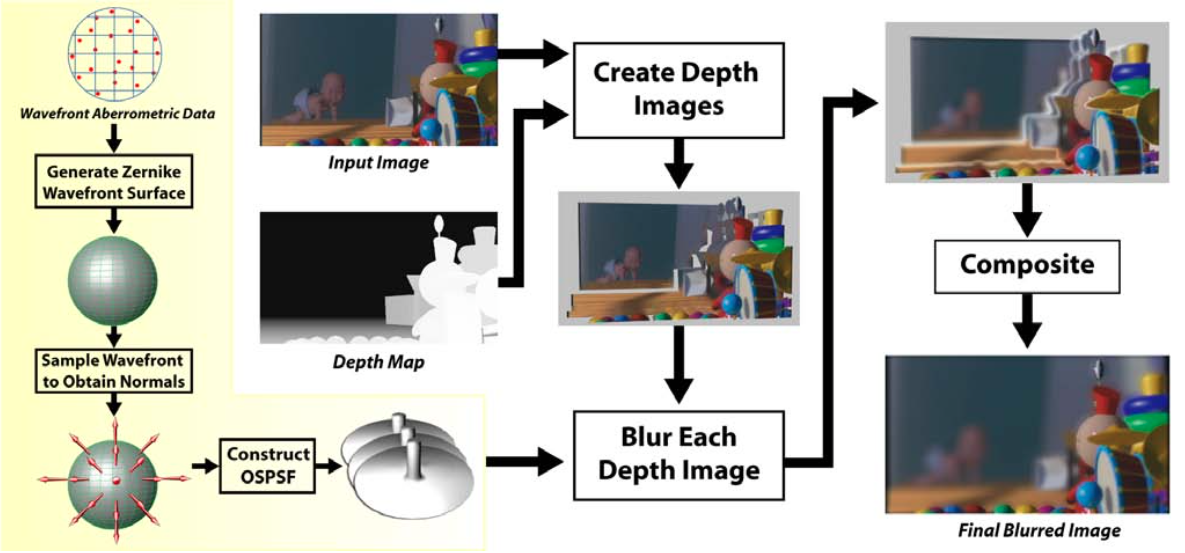
\includegraphics[width=0.99\linewidth]{__Images/03/barsky_pipeline.png}
	\caption[Overview of the vision-realistic rendering algorithm]{Overview of the vision-realistic rendering algorithm proposed by \citet{Barsky2004}. Given an individual's wavefront data and some synthetic scene, one can
	%one can compute the deviation from where the centroids would be in for an ideal wavefront; 
	generate millions of samples necessary to calculate an OSPSF; create a set of depth images; blur each depth image; and composite them to obtain a final blurred image.}
	\label{fig:barsky_algorithm}
\end{figure}

Many researchers have used raytracing techniques and anatomical optics to study and simulate vision by using theoretical models of the human eye \cite{Camp1990, Kolb1995}. \citet{Camp1990} described two ray tracing algorithms for deriving an optical PSF from corneal topography measurements. They focused on simulating and evaluating optical performance of patients' eyes with the following corneal pathologies: \emph{keratoconus}, \emph{epikeratophakia for aphakia} and \emph{radial keratonomy}. \citet{Kolb1995} presented a physically-based camera model that simulates aberration and radiation. To simulate such effects, they compute the geometry of image formation of a particular lens system using a modified distributed ray tracing algorithm. The algorithm is a hybrid of rendering and lens maker techniques, and can produce images of synthetic scenes showing a variety of optical effects. \citet{Mostafawy1997} combined the algorithm presented by \citet{Kolb1995} and the dimensions of an schematic eye model to generate virtual simulations of vision after corrective surgery.

\begin{figure}[!b]
	\centering

	\subfigure[Shack-Hartmann device's output]{
		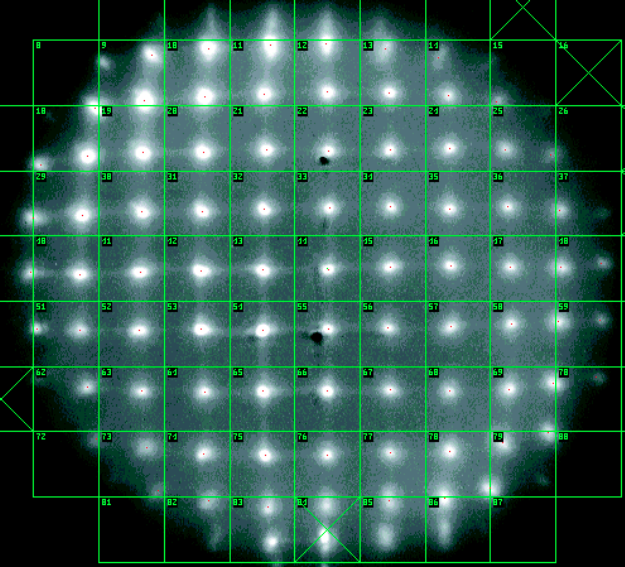
\includegraphics[width=140, height=140]{__Images/03/shackhartmann.png}
		\label{fig:yuA}
	}
	~
	\subfigure[Focused at infinity]{
		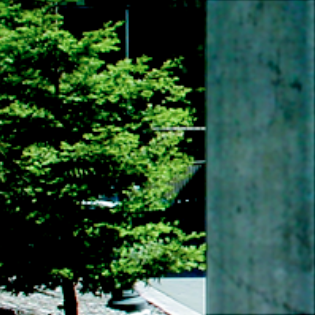
\includegraphics[width=140, height=140]{__Images/03/focused_atInf.png}
		\label{fig:yuB}
	}
	~
	\subfigure[Focused at 0.5m]{
		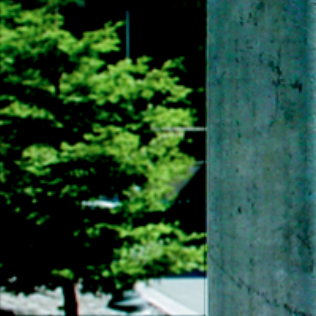
\includegraphics[width=140, height=140]{__Images/03/focused_atX.png}
		\label{fig:yuC}
	}
	
	\caption{\citet{Yu2001} uses data captured using a Shack-Hartmann aberrometer (a) to simulate blur at specific depth values (b) and (c).}
	\label{fig:yu}
\end{figure}

Moreover, the study of monochromatic aberrations of the human eye with wavefront sensors \cite{Liang1994} allowed many others to perform simulations by using Fourier tools to mimic visual perception. \citet{Yu2001} presents a technique capable of generating simulations of synthetic and  real scenes focusing at a specific depth (Figures~\ref{fig:yuB} and \ref{fig:yuC}). Instead of considering only the corneal surface and using raytracing techniques to perform such simulations, the authors rely on data captured by a Shack-Hartmann device (Figure~\ref{fig:yuA}). With this information they construct a wavefront, which is used to blur a sharp image according to a depth map. However, they do not present a proper way of evaluating the simulations' outcomes, which could be, for example, compared with an optical ground truth. 
\citet{Watson2008} proposed an image-based model for predicting acuity from optical aberrations. In this model, a `neural image' is computed incorporating optical and neural filtering. Then, this image is presented to four human observers and the LogMAR acuity is evaluated. By doing this, they can relate visual acuity as a function of a particular aberration and compute predictions of how a specific aberration (\eg, defocus) affects visual acuity.

%\textcolor{red}{NAO BASTA MENCIONAR OS OUTROS TRABALHOS. VOCE PRECISA DEIXAR CLARA AS DIFERENCAS ENTRE O QUE VOCE ESTÁ PROPONDO E O QUE OS OUTROS FIZERAM.}

	% Non-Optical Simulation Techniques Section
	% !TEX root = ./../../_Thesis.tex

% section's Name and Label
\subsection{Non-Optical Simulation Techniques}
\label{subsec:NonOpticalSimulationTechniques}

Some techniques are concerned with modeling the effects caused by non-optical issues and use them to achieve more realistic synthetic images. One example is the method proposed by \citet{Deering2005}. His approach describes a retinal photon-accurate model of the human eye. Such a model is used together with computer graphics techniques and a simplified eye's optical model to produce synthetic simulations of the image formation process. 

Another technique that explores different effects caused by the anatomy of the human eye --- the glare --- is discussed by \citet{Ritschel2009}. The authors proposed a model for a real-time dynamic simulation of the scattering in the human eye (Figure~\ref{fig:ritschel_pipeline}), which is efficiently implemented by drawing a few basic primitives, applying an FFT, and doing a special kind of blur. They have also performed psychophysical studies to measure the perception of brightness for glare models. However, they state that, as any other intrinsic phenomena, no ground truth can be obtained. And the model's validation remains a challenging task.

\begin{figure}[h]
	\centering
	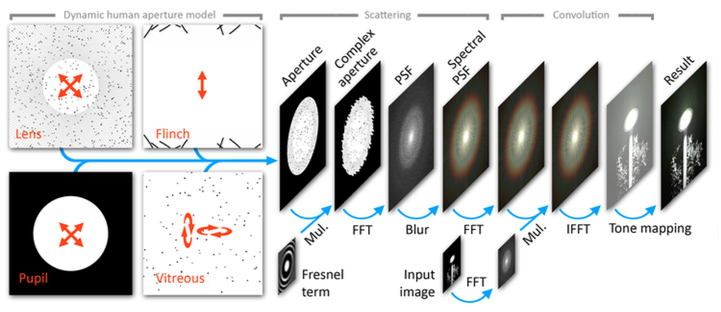
\includegraphics[width=0.99\linewidth]{__Images/03/ritschel_pipeline.png}
	\caption[The temporal glare pipeline]{The temporal glare pipeline \cite{Ritschel2009}.}
	\label{fig:ritschel_pipeline}
\end{figure}

% Estimating/Correcting Visual Optical Aberrations Section
% !TEX root = ./../../_Thesis.tex

% section's Name and Label
\section{Estimating/Correcting Visual Optical Aberrations}
\label{sec:EstimatingCorrectingVisualOpticalAberrations}

\citet{Pamplona2010} presented a practical approach for estimating low-order aberrations without the need of expensive equipments. It uses a pinhole mask attached to a smartphone displaying patterns to the subject. The aberrations are estimated by the subjective alignment of the different patterns.
\citet{Kronbauer2011} developed a psychophysical approach for vision measurement in candelas. It consists in presenting light stimulus in a display in order to discover the absolute threshold for clear and dark conditions. Then, by relating it with an objective vision's assessment (\eg, vision chart acuity and aberrometry data), they have stated a strong correlation between aberrometry data and the absolute threshold.

Many methods have achieved the goal of free the viewer from needing wearable optical correction when looking at displays \cite{Huang2012, Pamplona2012b, Huang2014}, and printings or projections \cite{Montalto2015}. Other works have explored physiologically-based models to provide insights and feedback on how to produce high-fidelity effects and improve visualization experiences \cite{Machado2009, Pamplona2009, Pamplona2011}.  

%\textcolor{red}{In fact, this kind of models has been widely used for different applications, such as 3D eye-model generation \cite{Berard2014}, improvements in individuals' accessibility \cite{Flatla2011}, and biometric authentication based on the iris \cite{Yano2012}. (?)}

% XYZ Section
% % !TEX root = ./../../_Thesis.tex

% section's Name and Label
\section{Image Filtering}
\label{sec:Image Filtering}

Given $S$, $C$, $R$, and $\phi$,  
one can obtain the effective aberration function as $kW_{(x,y)}$, where $k$ is the spherical wavenumber (\ie, $k = 2\pi/\lambda$), and 
$W_{(x,y)}$ is the wavefront aberration function expressed using the Zernike polymials. For the case of low-order aberrations, $W_{(x,y)}$ is defined by Equation~\ref{eq:W}, which takes into account oblique astigmatism, defocus, and vertical astigmatism. 
%\begin{equation}
%W_{(x,y)} = \sum_{i=-1}^1 c_{2}^{2i} \, Z_{2}^{2i}_{(x,y)}.
%\end{equation}
 $\lambda = 550nm$ is a standard wavelength used for monochromatic simulation \cite{Dai2008}.
 The pupil function $P_{(x,y)}$ is a binary  function that evaluates to 1 inside the projected aperture, and 0 outside it. According to \citet{Goodman2005}, the {\it generalized pupil function} $\mathbb{P}_{(x,y)}$ is given by:
\begin{equation}
	\centering
	\label{eq:generalizedpupilf}
	\mathbb{P}_{(x,y)} = P_{(x,y)} \exp[j*k*W_{(x,y)}],
\end{equation}
%
where $j = \sqrt{-1}$. Note that $\mathbb{P}_{(x,y)}$ is a complex number. One can obtain the point spread function of the optical system as the power spectrum of $\mathbb{P}$, \ie,  $PSF = \left | \mathcal{F}(\mathbb{P}) \right | ^ {2}$, where $\mathcal{F}$ is the Fourier transform operator.  Given the PSF and 
an input image $I$, one can simulate the view of $I$ through the given optical system computing the 2-D convolution
$O = PSF \otimes I$.
% and compute the two-dimensional convolution of $I$ and $\overline{PSF}$ in order to obtain the output image $O$. This is the simpler path for computing retinal images of a Sloan letter $S$ for a fixed depth, carried out entirely in the spatial domain. 
A more efficient computation of $O$ can be obtained in the frequency domain (this is illustrated by purple arrows in Figure~\ref{fig:roadmap}). In that case, $O = \mathcal{F}^{-1}(\mathcal{F}(I) * OTF)$, where $OTF = \mathcal{F}(PSF)$ is the {\it the optical transfer function} and $*$ is the element-wise multiplication. 
%
%the product of the object spectrum $\mathcal{F}(I)$ and the optical transfer function $OTF = \mathcal{F}(PSF)$ is the image spectrum, from which the image itself can be obtained by inverse Fourier transform $\mathcal{F}^{-1}(I * \overline{PSF}).

% XYZ Section
% % !TEX root = ./../../_Thesis.tex

% section's Name and Label
\section{Validation}} 
\label{sec:Validation}

To validate the visual simulation results of the refractive errors, we use a DSLR camera (Canon model EOS Rebel T3 with an 18-55mm zoom lens). The camera represents a perfect eye (\ie, without refractive aberrations). We place additional lenses in front of the camera's optical system to induce low-order aberrations (\ie, myopia, hyperopia, and astigmatism). Such lenses are placed on a support fixed to a UV filter attached to the main lens. Figure~\ref{fig:extralens} shows the camera with an additional +1.0 diopter lens attached to it. The support can hold up to three additional lenses. 
%
%results from the image filtering process, we've used additional lenses to induce low-order aberrations (\ie, myopia, hyperopia, and astigmatism) into the DSLR camera's optical system (Figure~\ref{fig:extralens}). 

For our simulations, we use a simplified eye model adjusted to the camera's settings to achieve consistent results between them.
% with the ones captured by the camera. 
More specifically, we make sure that the \emph{f-number} (\ie, the ratio of the camera lens' focal length $f$ to the diameter $D$ of its aperture):
\begin{equation}
	\centering
	\label{eq:fnumber}
	f_{number} = \frac{f}{D}
\end{equation}
\noindent
is the same for the camera and the eye model. For the experiments shown in the thesis, we fixed the focal length of the camera's main lens to 18mm (regardless of the use of additional lenses).
% to captured images (with or without extra lenses) with 18mm focal length and 
Thus, for instance, given \emph{f-number} values of $4.0$, $4.5$ and $5.0$, the corresponding camera lens aperture values are
%entrance pupil for each possible combination is
 4.5mm, 4.0mm and 3.6mm, respectively. 
Our simplified eye model (Figure~\ref{fig:syntheticeye}) has an axial diameter of 18mm. The crystalline lens causes the nodal point {\bf N} to be behind the crystalline. Thus, the eye model's effective focal length is 13.5mm: $f_{eye} = 18mm / \eta_{eye} =  18mm / 1.333 = 13.5 mm$, where $\eta_{eye}$ is the index of refraction of the eye. As a result, the eye model's pupil size (equivalent of the camera's lens aperture) needs to be rescaled to maintain the same \emph{f-number} value as the camera. Table~\ref{table:pupildiameter} shows the corresponding values of the equivalent camera apertures and pupil diameters. The simulation results shown in Chapter~\ref{chap:Results} were obtained for $f/5.0$ (third row of Table~\ref{table:pupildiameter}), although other values could have been used. 

%we must rescale the entrance pupil's diameter (Table~\ref{table:pupildiameter}) in order to maintain the same \emph{f-number} in simulations of retinal images. 

\begin{table}[h]
	\centering
	\caption{Camera apertures and pupil diameters for various f-numbers.}
	\label{table:pupildiameter}
	\begin{tabular}{rcc}
		\multicolumn{1}{l}{\bf f-number} & {\bf DSLR Camera (18mm focal length)} & {\bf Synthetic Eye (13.5mm focal length)} \\
		{\bf }               & {\bf aperture}     & {\bf pupil diameter}     \\
		{\bf $f/4.0$}         & 4.5mm                    & 3.4mm                        \\
		{\bf $f/4.5$}         & 4.0mm                    & 3.0mm                        \\
		{\bf $f/5.0$}         & 3.6mm                    & 2.7mm                        
	\end{tabular}
\end{table}

\begin{figure}[h]
	\centering
	
	\subfigure[]{
		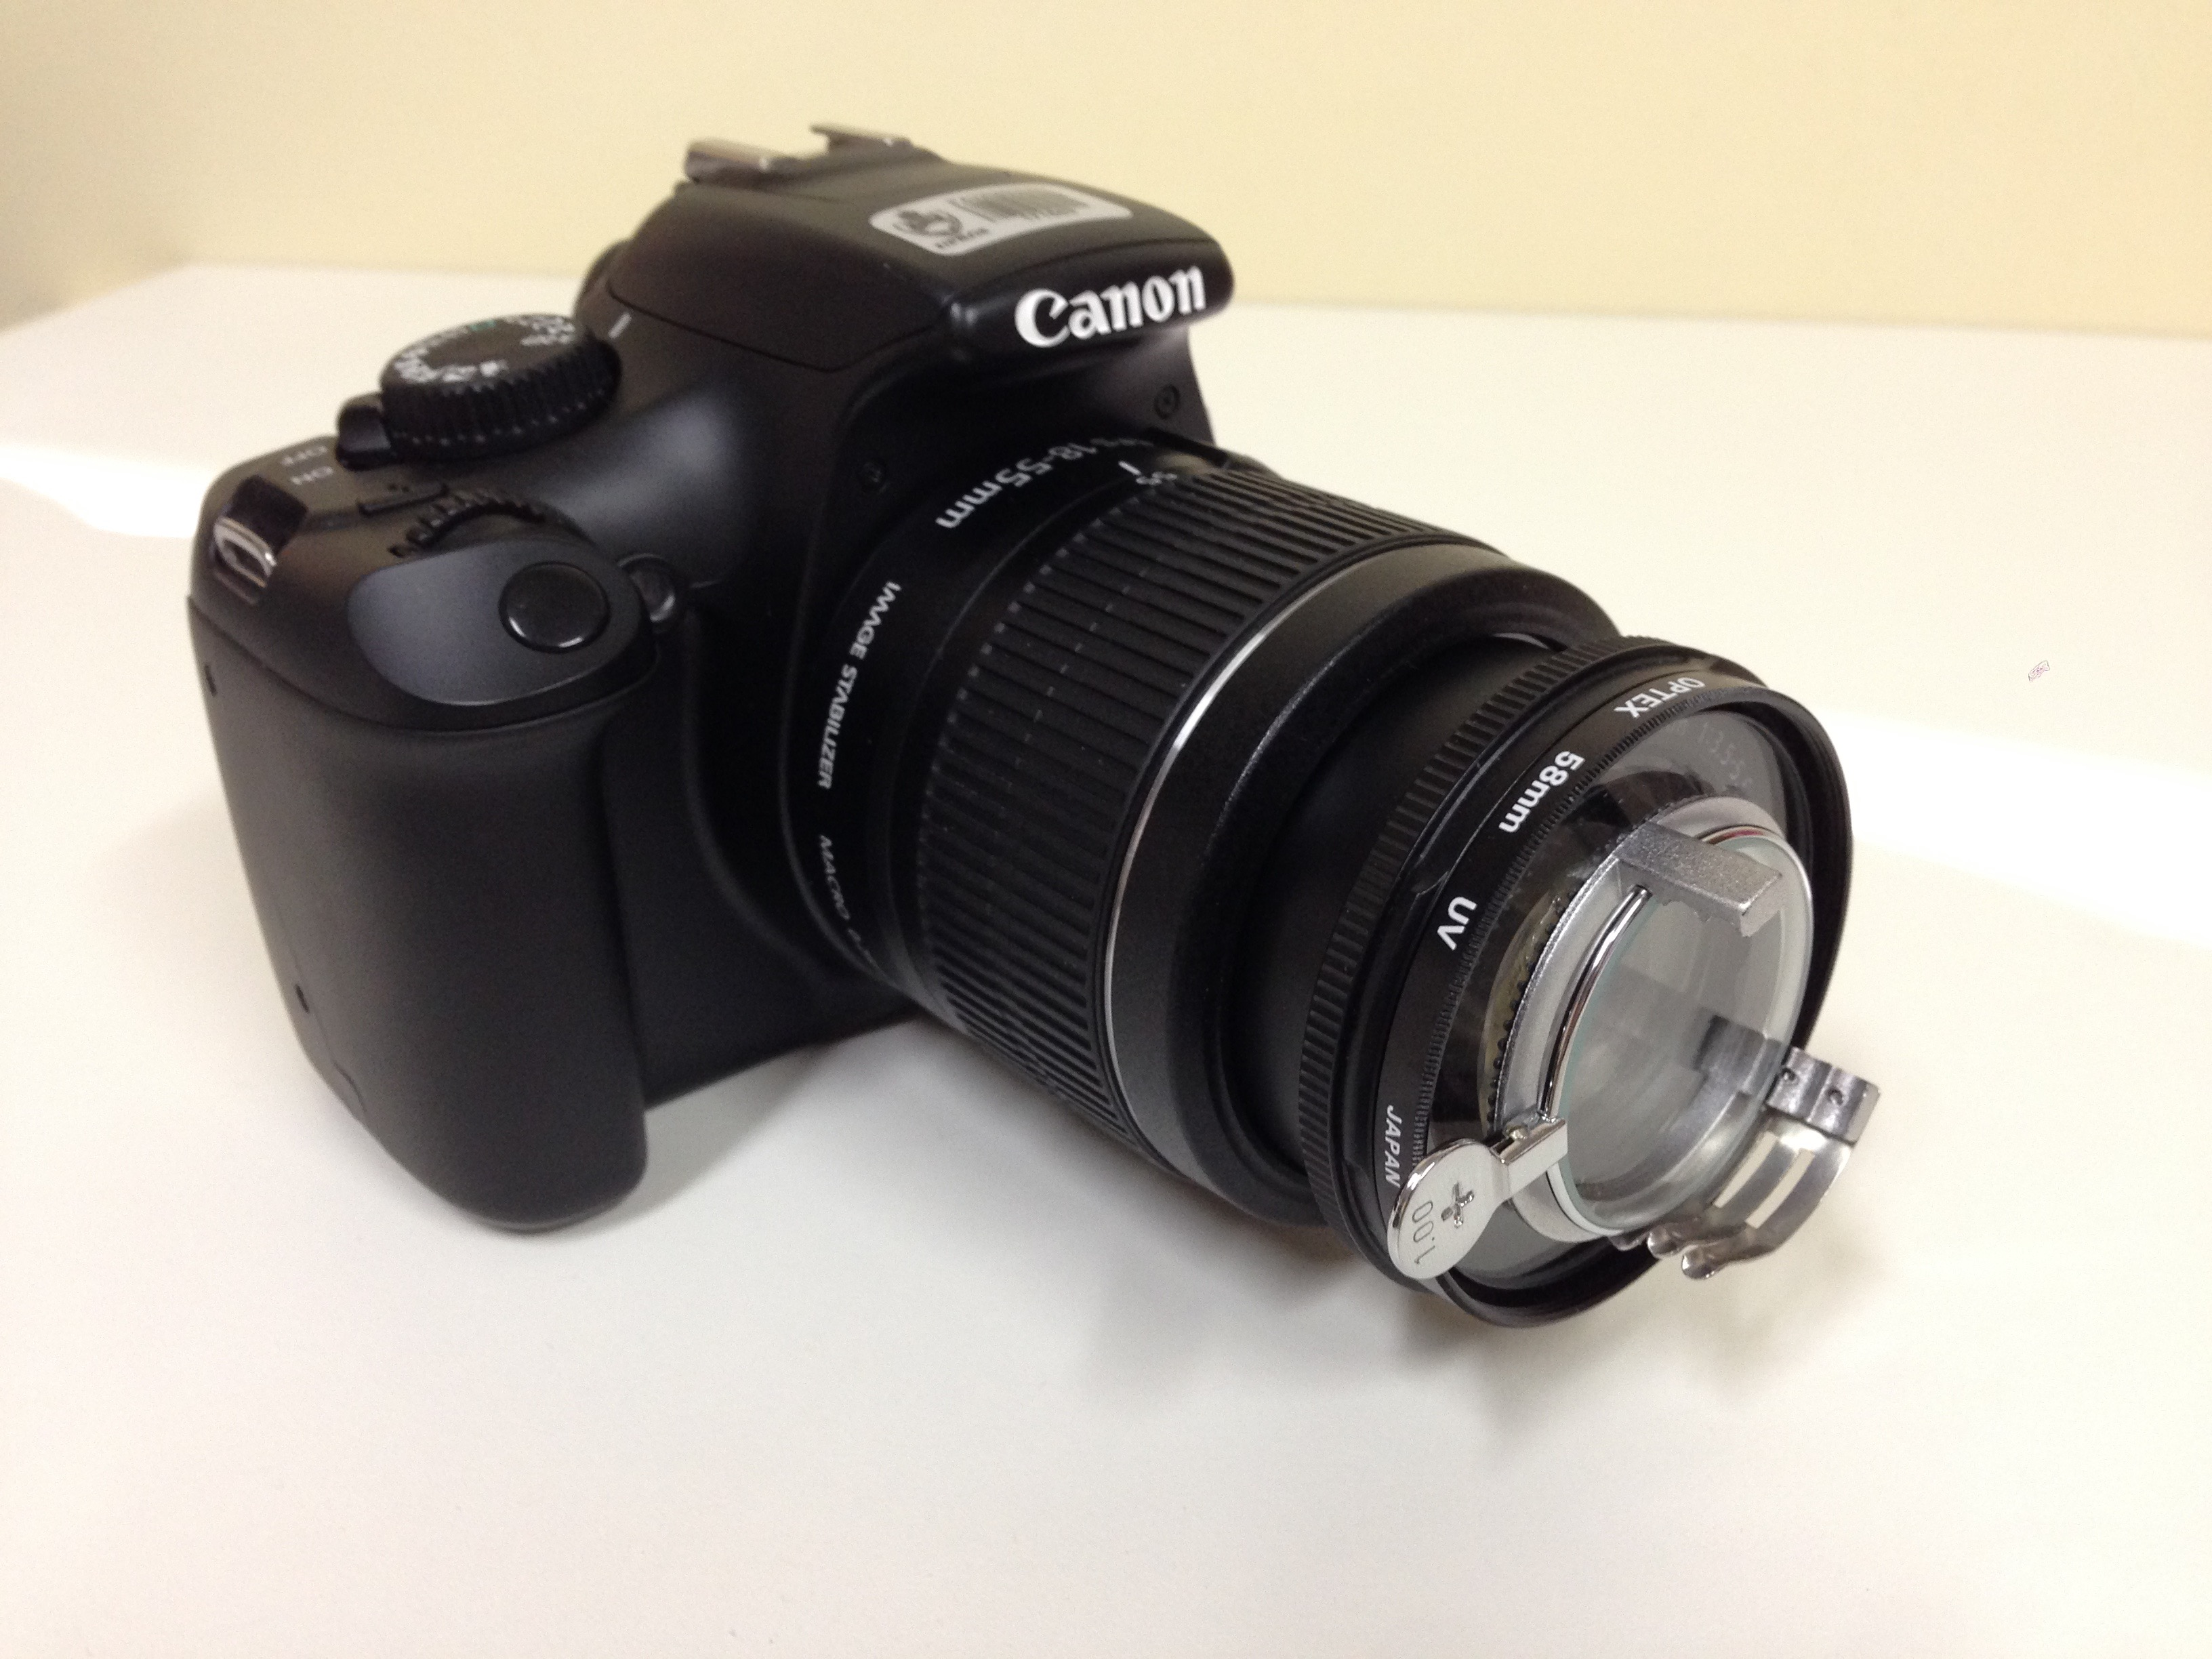
\includegraphics[width=0.55\linewidth]{__Images/04/camera.jpg}
		\label{fig:extralens}
	}
	~
	\subfigure[]{
		
\includegraphics[width=0.35\linewidth]{__Images/04/eyemodel.png}
		\label{fig:syntheticeye}
	}
	
	\caption[Optical systems used in the validation process]{Optical systems used in the validation process: (a) Canon EOS Rebel T3 with apparatus to add up to three extra lenses. Focal lens set to 18mm. (b) Simplified eye model with effective focal length of 13.5mm. {\bf N} is the nodal point.}
	\label{fig:camera}
\end{figure}

% XYZ Section
% % !TEX root = ./../../_Thesis.tex

% section's Name and Label
%\section{Absolute Threshold}
%\label{sec:AbsoluteThreshold}

In addition to the previously discussed optical aberrations that affect visual perception, there are non-optical characteristics (\ie, intrinsic individual phenomena) that could be considered in the simulation to achieve more realistic renderings of retinal images. In this section, we discuss an attempt to estimate one such intrinsic characteristic --- the {\it absolute threshold for vision} or simply {\it absolute threshold} or  
{\it minimum visible}.  
%(also known as the {\it minimum visible}) %with optical aberrations values. 
%Also, we try to integrate it in the optical simulation pipeline. 
%When an imaging system (\eg, the human eye) is mis-focused at a point in the scene, 
The light emitted/reflected by an out-of-focus scene point is spread out across some area of the observer's retinal surface, producing a so-called {\it circle of confusion} and causing blur (Figure~\ref{fig:coc}). Since the eye's photoreceptors have an energy threshold for triggering a neural signal indicating light detection, the larger the circle of confusion (and consequent spread of the incoming energy), the bigger should be the light intensity required to trigger such neural signal. Thus, considering an individual without any condition that reduces the translucency of the eye along its optical path (\eg, cataracts), we have formulated the following hypothesis: 

\vspace{0.2cm}
\noindent
{\bf H1}:
%By considering this statements, we've created the following hypothesis:
{\it The absolute threshold for vision is directly proportional to the magnitudes of the eye's defocus (\ie, myopia or hyperopia) and astigmatism.
As such, the absolute threshold can be used as an estimate of the spherical equivalent of the eye's refractive error}. 
\\

The {\it spherical equivalent} is the sum of the spherical (defocus) plus half of the cylindrical (astigmatism) values of the optical system (\ie, $S + 0.5 \times C$) expressed in diopters.

\begin{figure}[h]
	\centering
	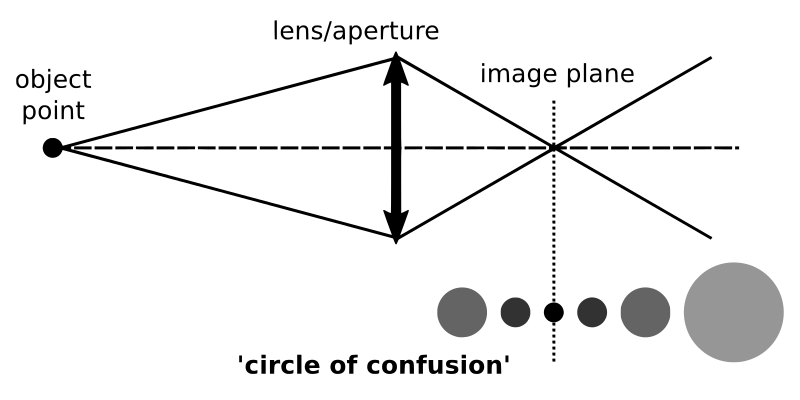
\includegraphics[width=0.6\linewidth]{__Images/04/mv_insight.png}
	\caption[Geometrical perspective of the circle of confusion]{The image of an in-focus point is formed on the image plane. An out-of-focus point, on the other hand, projects a so-called circle of confusion on the image plane, causing blur. The radius of the circle is proportional to the amount of defocus.} 
%	Geometrical perspective of the circle of confusion}
	\label{fig:coc}
\end{figure}

The following subsections discuss a psychophysical experiment established to estimate the absolute threshold information of an eye. The population sample is presented together with the quasi-random algorithm used during the experiments. 
%Finally, we detail a simple way for generating retinal images deeming this specific non-optical aberration.